\documentclass[12pt]{article}%
\usepackage{graphicx}
\usepackage{ragged2e}
\usepackage{indentfirst}
\usepackage{float}
%\usepackage{setspace}
%\usepackage{subfigure}
%\usepackage{amsmath}
%\usepackage{amsfonts}
%\usepackage{amssymb}
%\usepackage{amsbsy}
%\usepackage{times}
\usepackage[colorlinks=true,citecolor=black,linkcolor=black]{hyperref}
%\usepackage{multirow}
%\usepackage{booktabs}
\usepackage[english]{babel}
\usepackage[utf8]{inputenc}
\usepackage{fancyhdr}
%
\pagestyle{fancy}
\fancyhf{}
\rhead{Spring 2017}
\lhead{CALVIN \& PyVIN Shortcourse}
\cfoot{\thepage}
\rfoot{\textit{\small updated on \today}}
% 
\begin{document}
%
\title{\textbf{CALVIN \& PyVIN} Shortcourse}
%
\date{April 1, 2017}
\author{
Mustafa S. Dogan
%
\thanks{
Graduate Student,
Dept.\ of Civil and Env. Eng.,
Univ.\ of California, Davis, 
1 Shields Avenue,
Davis, CA  95616. E-mail: msdogan@ucdavis.edu.},
}
%
\maketitle
%
\tableofcontents
%
\pagebreak
%
\begin{center}
	{\bf \Huge{Agenda and Topics \\}}
\end{center}
%
\hrule
\begin{table}[h]
    \centering
    %\caption{\huge agenda & topics}
    \label{agenda}
    \begin{tabular}{lll}
         15 min &\textendash & Introduction and set-up \\
         1 hr &\textendash & CALVIN theory and model introduction \\
         \bf{15 min} &\textendash & \bf{Break} \\
         15-20 min &\textendash & HOBBES database \\
         15 min &\textendash & Data flow overview \\
         \bf{1 hr} &\textendash & \bf{Break} \\
         20-25 min &\textendash & PyVIN updates and model architecture\\
         15 min &\textendash & A PyVIN example \\
         \bf{15 min} &\textendash & \bf{Break} \\
         15-20 min &\textendash & Required software and installation \\
         20 min &\textendash & Your first PyVIN run \\
         20-25 min &\textendash & Postprocessing results
    \end{tabular}
\end{table}
\hrule
%
\pagebreak
\section{Prerequisites}
Please bring your \textbf{laptop} with below software dependencies installed if you want a hands-on PyVIN experience. Install following software in advance since some of them, such as Anaconda, takes long time to download and install. If you have any question, e-mail msdogan@ucdavis.edu
%
\begin{itemize}
	\item {\bf Python v3 with Anaconda} \\ Link: https://www.continuum.io/downloads
	\begin{figure}[H]
		\centering
    		\includegraphics[width=0.5\linewidth]{anaconda.pdf}
   		\caption{Anaconda package for Windows and Mac OS}
    		\label{fig:anaconda}
	\end{figure}
	Note: Download Python v3+ (not v2.7) because Pyomo command line installation works only with Python v3+
	\item {\bf GitHub} \\ Link: https://desktop.github.com
	\begin{figure}[H]
		\centering
    		\includegraphics[width=0.45\linewidth]{github.pdf}
   		\caption{GitHub installation for Windows and Mac OS}
    		\label{fig:github}
	\end{figure}
	\item {\bf Pyomo} \\ Command: {\tt \small conda install -c cachemeorg pyomo pyomo.extras glpk}
\end{itemize}
%
Note: if you don't know how to use command line, please refer to description below and then type the command.
\subsection{Command line}
%
This shortcourse is not intended to explain command line use. It assumes some but not extensive command line knowledge. If you like to learn basics of command line, here is a nice crash course:
%
\par https://learnpythonthehardway.org/book/appendixa.html
%
\begin{figure}[H]
    \centering
    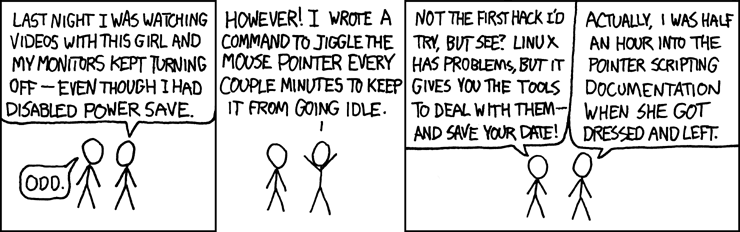
\includegraphics[width=1\linewidth]{command_line_fu.png}
    \caption{A command line comic from xkcd, source: https://xkcd.com/196/}
    \label{fig:command_line}
\end{figure}
%
\subsubsection{Windows}
%
After installing GitHub, double click on "Git Bash" and then type the command above to install Pyomo and GLPK solver.
\subsubsection{Mac OS}
%
Search "terminal" in Spotlight Search and then double click. Type the command above to install Pyomo and GLPK solver.
\begin{figure}[H]
		\centering
    		\includegraphics[width=0.6\linewidth]{terminal.pdf}
   		\caption{Command line (terminal) for Mac OS}
    		\label{fig:terminal}
	\end{figure}
%
\pagebreak
%
\section{Introduction and background}
%
Developed in early 2000s, {\bf CAL}ifornia {\bf V}alue {\bf IN}tegrated model (CALVIN) combines ideas from economics and engineering optimization with advances in software and data to suggest more integrated management of water supplies regionally and throughout California. CALVIN is an hydro-economic optimization model for California's advanced water infrastructure that integrates the operation of water facilities, resources, and demands, and it aims to optimize surface and groundwater deliveries to agricultural and urban water users. It allocates water to maximize statewide agricultural and urban economic value, considering physical and policy constraints. It replicates water market operations transferring water from users with lower willingness-to-pay to users with higher willingness-to-pay. CALVIN uses historical hydrology and 2050 water demand projections for its operations. Figure \ref{fig:coverage} regions and coverage of the model. \\
\par CALVIN forces quantitative understanding of integrated water and economic system. Motivation for the CALVIN effort include:
\begin{itemize}
	\item making better sense of integrated system and operations
	\item seeking ways to improve system management
	\item quantifying user willingness to pay for additional water
	\item finding insights into changes in physical capacities and policies
\end{itemize}
%
\par With the recent updates, CALVIN is evolved to open-source PyVIN model, optimizing water resources in a short amount of time with state-of-the-art solvers and modeling platform. PyVIN has the same input data and objective as CALVIN but it is modeled on Pyomo, a Python-based high level algebraic modeling language. PyVIN also uses HOBBES database, which allows better documentation, collaboration and communication between models as well as modelers.
%
\begin{figure}[H]
    \centering
    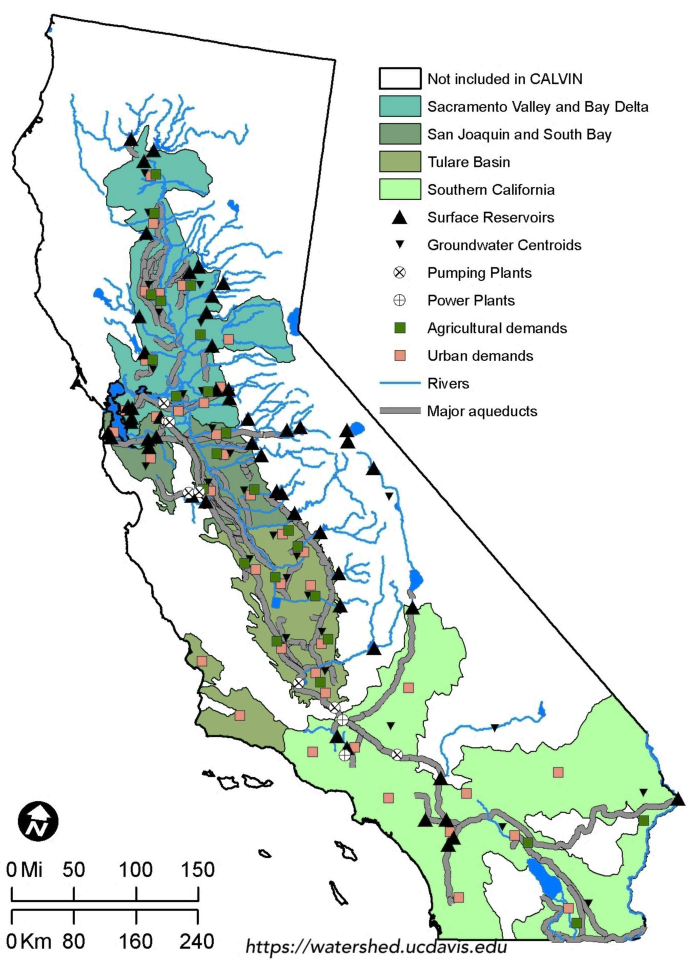
\includegraphics[width=0.9\linewidth]{coverage.pdf}
    \caption{California's water infrastructure and CALVIN's coverage}
    \label{fig:coverage}
\end{figure}
%
\section{HOBBES database}
%
\section{Structure}
%
\section{Updated version: PyVIN}
%
\subsection{new version}
%
\subsection{software requirements}
%
\subsection{first model run}
%
\section{References and useful links}
\end{document}